% !TEX program = pdflatex
\documentclass[conference]{IEEEtran}
\IEEEoverridecommandlockouts

\usepackage{cite}
\usepackage{amsmath,amssymb,amsfonts}
\usepackage{algorithm}
\usepackage{algorithmic}
\usepackage{graphicx}
\usepackage{textcomp}
\usepackage{xcolor}
\usepackage{tikz}
\usetikzlibrary{arrows,positioning,calc,shapes.geometric,fit,arrows.meta}
\usepackage{booktabs}
\usepackage{array}
\usepackage{url}
\usepackage[hidelinks]{hyperref}
\usepackage{float}
\usepackage{caption}
\renewcommand{\thetable}{\arabic{table}}
\makeatletter
\long\def\@makecaption#1#2{%
\@IEEEfigurecaptionsepspace
\setbox\@tempboxa\hbox{\normalfont\footnotesize {#1.}\nobreakspace\nobreakspace #2}%
\ifdim \wd\@tempboxa >\hsize%
\setbox\@tempboxa\hbox{\normalfont\footnotesize {#1.}\nobreakspace\nobreakspace}%
\parbox[t]{\hsize}{\normalfont\footnotesize\noindent\unhbox\@tempboxa#2}%
\else%
\ifCLASSOPTIONconference \hbox to\hsize{\normalfont\footnotesize\hfil\box\@tempboxa\hfil}%
\else \hbox to\hsize{\normalfont\footnotesize\box\@tempboxa\hfil}%
\fi\fi}
\makeatother
\usepackage{listings}
\lstset{
  language=Java,
  basicstyle=\ttfamily\tiny,
  columns=fullflexible,
  keepspaces=true,
  breaklines=true,
  breakatwhitespace=false,
  frame=single,
  numbers=left,
  numberstyle=\tiny,
  numbersep=2pt,
  xleftmargin=0pt,
  framexleftmargin=4pt,
  linewidth=\columnwidth,
  aboveskip=6pt,
  belowskip=4pt,
  abovecaptionskip=6pt,
  belowcaptionskip=4pt,
  framexbottommargin=4pt,
  captionpos=b,
}

\renewcommand{\dbltopfraction}{0.9}
\renewcommand{\dblfloatpagefraction}{0.8}
\renewcommand{\topfraction}{0.9}
\renewcommand{\floatpagefraction}{0.8}
\setcounter{dbltopnumber}{4}

\def\BibTeX{{\rm B\kern-.05em{\sc i\kern-.025em b}\kern-.08em
    T\kern-.1667em\lower.7ex\hbox{E}\kern-.125emX}}

\begin{document}

\title{\vspace*{1cm} Dependency-Aware Code Smell Refactoring with an Adaptive Coding-Agent Harness}

\author{
\IEEEauthorblockN{Havriil Pietukhin}
\IEEEauthorblockA{\textit{Department of Applied Informatics} \\
\textit{Faculty of Mathematics, Physics and Informatics,}\\
\textit{Comenius University in Bratislava}\\
0009-0000-7504-9720\\
pietukhin1@uniba.sk}
\and
\IEEEauthorblockN{Ivan Pol\'{a}\v{s}ek}
\IEEEauthorblockA{\textit{Gratex International,}\\
\textit{Department of Applied Informatics} \\
\textit{Faculty of Mathematics, Physics and Informatics,}\\
\textit{Comenius University in Bratislava}\\
0000-0001-6004-701X\\
ipo@gratex.com}
}

\maketitle

\begin{abstract}
Refactoring one code smell can remove or introduce others, so operation order
matters. We extend a coding-agent harness with dependency-aware planning,
Java editing, and an automatic verification loop. Each Java edit triggers the
project tests and the Organic smell detector. The harness returns both results
to the coding agent before it continues. A smell may receive five attempts. The
harness changes from a low-cost model to a stronger model after two failed
attempts. We evaluate four ordering methods on executable Java episodes
reconstructed from the Neo4j representation of the Sousa composite-refactoring
dataset. Across 20 completed runs, the harness removed all 350
initial smell detections and all 220 detections introduced during editing.
Compilation failed during 171 of 704 intermediate verifications, and 14 runs
had at least one failure. The harness recovered from these intermediate
failures, but its edits were not error-free. For the episodes evaluated with
Best-First Search, it
introduced fewer smells than detector order and required fewer edit tasks than
topological ordering.
\end{abstract}

\begin{IEEEkeywords}
code smells, automated refactoring, coding agents, search-based software
engineering, static analysis
\end{IEEEkeywords}

%----------------------------------------------------------------------
\section{Introduction}
%----------------------------------------------------------------------

Code smells~\cite{Fowler1999} are symptoms of poor object-oriented design.
In long-lived projects, they accumulate, make code harder to read, and raise
maintenance cost.
More than 59\% of smell-bearing classes contain multiple
smells~\cite{palomba2018diffuseness}. Combined smells hurt comprehension much
more than isolated smells~\cite{abbes2011empirical}.
Recent large language model (LLM)-based tools automate individual
refactorings~\cite{10.1145/3691620.3695508,liang2025smelldetector}, but they
usually treat each smell independently.

Cedrim et al.~\cite{cedrim2017} found that 57\% of refactorings in a
longitudinal study of 23 Java projects did not reduce the smell count; some
increased it.
Operation order matters because smells interact. Refactoring one smell can
remove or introduce others, depending on the current class structure.
Markovič~\cite{markovic2016refaktorovanie} formalised these positive and
negative dependency rules.
We use that catalogue for dependency candidates, restricted to the smell types
and refactoring operations listed in our tables.

We study four questions.

\textbf{(RQ1) Planner choice.} How does the planning algorithm affect whether
the harness removes all detected smells while the repository tests pass?

\textbf{(RQ2) Dependency rules.} How do the positive and negative dependency
rules affect the same outcome?

\textbf{(RQ3) Predicted and observed dependencies.} Do different planners
produce the smell removals and introductions predicted by the rule catalogue?

\textbf{(RQ4) Structural quality.} How do the resulting code states differ in
CBO, LCOM, WMC, and LOC?

Our implementation extends a coding-agent harness. It builds a directed
dependency graph, orders detected smells, asks the coding model to edit one
smell at a time, and checks each edit before continuing. Its control loop
returns test and detector results to the coding model before selecting the next
smell. The ordering algorithms use the same dependency graph.

%----------------------------------------------------------------------
\section{Related work}
%----------------------------------------------------------------------

\subsection{Code smell detection}

Lanza and Marinescu~\cite{lanza2006object} systematised threshold-based
detectors built on the metrics of Chidamber and Kemerer~\cite{chidamber1994metrics}.
Fontana et al.~\cite{fontana2016comparing} reported 96\% SVM accuracy across 74
Java projects. Yamashita and Moonen~\cite{yamashita2013exploring} and Palomba
et al.~\cite{palomba2018diffuseness} studied co-located smells. Palomba et al.
found multiple smell types in 59\% of smell-bearing classes. Abbes et
al.~\cite{abbes2011empirical} measured a 124\% reduction in comprehension for
combined smells.

\subsection{Code refactoring}

Cedrim et al.~\cite{cedrim2017} annotated 16,566 refactorings in 23 projects as
smell-reducing, smell-introducing, or neutral. Of these operations, 57\% did not
reduce the smell count, and some increased it.
Execution order can decide whether automated refactoring improves or worsens a
codebase.
Markovič~\cite{markovic2016refaktorovanie} derived a catalogue of
positive dependencies (refactoring smell $A$ may resolve smell $B$ as a side
effect) and negative dependencies (refactoring $A$ may introduce $B$),
grounded in Fowler's refactoring catalogue~\cite{Fowler1999}.
Negative edges depend on state. A negative dependency applies only when the
class still has the required structure. Removing prerequisite smells first can
suppress the edge. The catalogue gives
candidate effects rather than measured probabilities. We use it to order
operations, then redetect smells after each actual edit.

\subsection{Large language models for code}

iSMELL~\cite{10.1145/3691620.3695508} combines Mixture-of-Experts with static
analysis and reports F1\,=\,75.17\% on seven smell types.
SmellDetector~\cite{liang2025smelldetector} (IJCNN~2025) fine-tunes LLMs for
multi-label smell detection across Java projects.
Both target individual smell instances; neither models interactions between
sequential refactoring operations or uses dependency-aware planning.

The coding harness also affects cost and task completion. Gaba et
al.~\cite{gaba2026databricks} ran the same model and reasoning effort through
several harnesses on internal Databricks tasks. Pi sent about one third as much
context per turn. Some configurations differed in cost by more than a factor of
two at equal measured quality. Their tasks differ from ours, so we use these
results only to justify the harness choice.

%----------------------------------------------------------------------
\section{Our Approach}
%----------------------------------------------------------------------

\subsection{Method overview}

The implementation uses Pi, a terminal coding-agent harness with a TypeScript
extension interface and model switching~\cite{pi2026}. In the Databricks
benchmark, Pi matched measured quality while reducing context use and, in some
configurations, cost~\cite{gaba2026databricks}.
Pi separates model access from agent execution and loads workflow changes
through extensions~\cite{pi2026}. Our extension prepares a dataset case,
presents one smell, monitors Java changes, runs verification, and returns the
result to the coding model. Fig.~\ref{fig:pipeline} shows this loop.

The dependency rules predict which smells one refactoring may remove or
introduce. DAPS, topological ordering, and BeFS use those predictions to select
the next smell. The harness requests the edit, checks it, reports failures, and
retries when needed. Organic then redetects the smells. Its output, not the
predicted transition, defines the next state.

\begin{figure*}[tb]
\centering
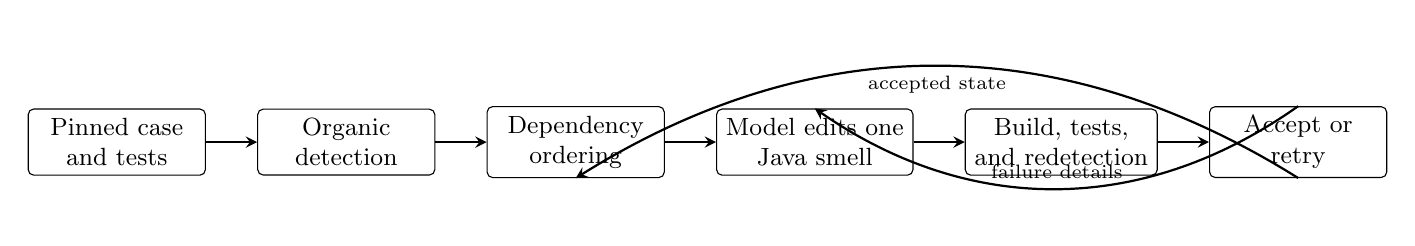
\begin{tikzpicture}[
  box/.style={draw, rounded corners=2pt, minimum width=2.25cm,
    minimum height=0.75cm, align=center, font=\small},
  arr/.style={->, >=stealth, thick},
  node distance=0.65cm]
  \node[box] (case) {Pinned case\\and tests};
  \node[box, right=of case] (detect) {Organic\\detection};
  \node[box, right=of detect] (plan) {Dependency\\ordering};
  \node[box, right=of plan] (edit) {Model edits one\\Java smell};
  \node[box, right=of edit] (verify) {Build, tests,\\and redetection};
  \node[box, right=of verify] (gate) {Accept or\\retry};
  \draw[arr] (case) -- (detect);
  \draw[arr] (detect) -- (plan);
  \draw[arr] (plan) -- (edit);
  \draw[arr] (edit) -- (verify);
  \draw[arr] (verify) -- (gate);
  \draw[arr, bend left=35] (gate.north) to
    node[above, font=\scriptsize]{failure details} (edit.north);
  \draw[arr, bend right=32] (gate.south) to
    node[below, font=\scriptsize]{accepted state} (plan.south);
\end{tikzpicture}
\caption{Modified coding-agent control loop. The detector and project tests
produce each accepted state; predicted planner transitions do not.}
\label{fig:pipeline}
\end{figure*}

The harness checks out the recorded start commit in an isolated worktree. The
Organic detector~\cite{organic2022} scans the selected classes and methods. A
task includes the smell type, severity, owner, source range, detector evidence,
and refactoring advice. The model receives only the current smell turn. The
harness uses the tests already present in each repository and does not generate
new tests.

\subsection{Smell dependency model}

We represent smell dependencies as a directed graph $G=(V,E)$, where each node
$s_i \in V$ is a detected smell instance.
The graph has two edge types:
\begin{itemize}
  \item \textit{positive} $s_i \xrightarrow{+} s_j$: refactoring $s_i$
        may resolve $s_j$ as a side effect;
  \item \textit{negative} $s_i \xrightarrow{-} s_j$: refactoring $s_i$
        may introduce $s_j$.
\end{itemize}
We add an edge when the smell-type pair matches a rule from the
catalogue~\cite{markovic2016refaktorovanie} and both smells are in the same
class context. A positive edge predicts that one refactoring may remove another
smell. A negative edge predicts that it may introduce one. These predictions
rank operations. After each Java edit, Organic replaces the predicted state
with detector output. We treat negative edges as more reliable because a
positive side effect may not occur in a given class. Positive edges use
co-located source instances. Negative edges use the abstract catalogue rules.
The model does not include transitive positive dependencies.
Table~\ref{tab:deps} lists the implemented rules.

\begin{table}[tb]
\caption{Dependency rules~\cite{markovic2016refaktorovanie}.}
\label{tab:deps}
\centering
\footnotesize
\setlength{\tabcolsep}{2.5pt}
\begin{tabular}{@{}p{2.0cm}p{2.6cm}p{2.6cm}@{}}
\toprule
\textbf{Smell} & \textbf{Positive (resolves)} &
  \textbf{Negative (introduces)} \\
\midrule
Long Method / Complex &
  Feature Envy, Dup.\ Code, Long Param.\ List &
  Long Method, Long Param.\ List \\
Long Param.\ List &
  Data Clumps &
  Data Class \\
God Class / Large Class &
  Feature Envy, Data Clumps &
  Long Method, Data Class, Inapp.\ Intimacy \\
Dup.\ Conditions &
  Divergent Change &
  Large Class \\
\bottomrule
\end{tabular}
\end{table}

\subsection{Refactoring-order algorithms}

The ordering algorithms give the harness one detected smell at a time.
Dependency-Aware Priority Selection (DAPS) assigns each smell $s_i$ a priority
score $P(s_i)$ and chooses the highest-scoring smell.
The general form is:
\begin{equation}
  \begin{split}
    P_i = f_i \cdot \bigl( &w_{\mathrm{sev}} \cdot \mathrm{sev}(s_i)
           + \textstyle\sum \mathrm{pos\_out}(s_i) \\
           &- w_{\mathrm{neg}} \cdot \textstyle\sum \mathrm{neg\_out}(s_i) \bigr),
  \end{split}
  \label{eq:p-general}
\end{equation}
where $f_i = \mathrm{freq}(s_i)$ counts occurrences of smell $s_i$.
$w_{\mathrm{sev}}{=}0.33$ normalises the severity scale.
$w_{\mathrm{neg}}{=}0.5$ discounts predicted introductions because they depend
on class structure. $\mathrm{pos\_out}$ and $\mathrm{neg\_out}$ count outgoing
positive and negative edges.

Positive edges require co-located smell instances in the source file. Negative
edges follow Markovič's abstract catalogue because their structural risk does
not depend on observed co-location.
The concrete priority formula is:
\begin{equation}
  \begin{split}
    P^{\mathrm{conc}}_i = f_i \cdot \bigl( &w_{\mathrm{sev}} \cdot \mathrm{sev}(s_i)
           + \textstyle\sum \mathrm{pos\_out}^{\mathrm{conc}}(s_i) \\
           &- w_{\mathrm{neg}} \cdot \textstyle\sum \mathrm{neg\_out}^{\mathrm{abs}}(s_i) \bigr).
  \end{split}
  \label{eq:p-concrete}
\end{equation}
Future calibration could weight each positive edge by its observed probability
using data such as that of Cedrim et al.~\cite{cedrim2017}.
DAPS selects $\arg\max P_i$ at each step. This local choice may produce a poor
global order when the selected smell has active negative edges.

\subsubsection{Topological ordering}
The topological treatment follows the scored ordering proposed by Orlova and
Polášek~\cite{orlova2026topological}. It converts dependency edges into
refactoring-preference constraints, condenses strongly connected components,
and scores candidate topological orders by positive-edge distance and vertex
weight. Our implementation enumerates at most 4,096 orders and selects the order
with the largest sum of normalised distance and vertex scores. It sends the
first smell in that order to the coding model.

\subsubsection{Dependency-Aware Priority Selection}
Algorithm~\ref{alg:daps} formalises DAPS.

\begin{algorithm}[tb]
\caption{Dependency-Aware Priority Selection (DAPS).}
\label{alg:daps}
\begin{algorithmic}[1]
\REQUIRE Initial state $S_0$, dependency rules $R$
\ENSURE Ordered refactoring plan $\pi$
\STATE $S \leftarrow S_0$;\quad $\pi \leftarrow [\,]$
\WHILE{$S \neq \emptyset$}
  \FOR{each $s_i \in S$}
    \STATE $P(s_i) \leftarrow f_i \cdot \bigl( w_{\mathrm{sev}} \cdot \mathrm{sev}(s_i)
             + \sum\mathrm{pos\_out}^{\mathrm{conc}}(s_i)$
    \STATE \hspace{2.6em} $- w_{\mathrm{neg}} \cdot \sum\mathrm{neg\_out}^{\mathrm{abs}}(s_i) \bigr)$
  \ENDFOR
  \STATE $s^* \leftarrow \arg\max_{s_i \in S} P(s_i)$
  \STATE $\pi \leftarrow \pi{+\!\!+}[r(s^*)]$
  \STATE $S \leftarrow (S \setminus \mathrm{resolved}(s^*,S)) \cup \mathrm{created}(s^*,S)$
\ENDWHILE
\RETURN $\pi$
\end{algorithmic}
\end{algorithm}

\subsubsection{Best-First Search (BeFS) algorithm}
Algorithm~\ref{alg:befs} treats refactoring as state-space search:
\begin{itemize}
  \item \textbf{State} $S$: current set of active smell instances;
  \item \textbf{Action} $r(s_i)$: refactor smell $s_i \in S$;
  \item \textbf{Transition}:
        $S' = (S \setminus \mathrm{resolved}(s_i, S))
               \cup \mathrm{created}(s_i, S)$,
        where $\mathrm{resolved}(s_i, S)$ includes $s_i$ itself plus any
        smells in $S$ that are positively resolved as a side effect;
  \item \textbf{Heuristic}: $h(S) = \sum_{s \in S} \mathrm{sev}(s)$;
  \item \textbf{Objective}: minimise $h(S)$; the search seeks the lowest
        achievable total severity, which need not reach zero.
\end{itemize}
BeFS orders states by $h(S)$, not by the per-smell priority $P(s_i)$. Only DAPS
uses this score to choose the next smell (Algorithm~\ref{alg:daps}).
The implementation stops after at most $N_{\max}{=}10{,}000$ state expansions.
The CLOSED set prevents revisiting an expanded state.

\begin{algorithm}[tb]
\caption{BeFS algorithm.}
\label{alg:befs}
\begin{algorithmic}[1]
\REQUIRE Initial state $S_0$, dependency rules $R$, expansion limit $N_{\max}$
\ENSURE Lowest-$h$ plan found within $N_{\max}$ expansions
\STATE $\text{OPEN} \leftarrow \{(h(S_0), S_0, [\,])\}$
\STATE $\text{CLOSED} \leftarrow \emptyset$;\quad $n \leftarrow 0$;\quad $\pi^* \leftarrow [\,]$;\quad $h^* \leftarrow h(S_0)$
\WHILE{$\text{OPEN} \neq \emptyset \land n < N_{\max}$}
  \STATE $(h, S, \pi) \leftarrow \text{extract\_min}(\text{OPEN})$
  \IF{$h < h^*$} \STATE $h^* \leftarrow h$;\quad $\pi^* \leftarrow \pi$ \ENDIF
  \IF{$S \in \text{CLOSED}$} \STATE \textbf{continue} \ENDIF
  \STATE $\text{CLOSED} \leftarrow \text{CLOSED} \cup \{S\}$
  \STATE $n \leftarrow n+1$
  \FOR{each $s_i \in S$}
    \STATE $S' \leftarrow (S \setminus \mathrm{resolved}(s_i,S))
                          \cup \mathrm{created}(s_i,S)$
    \IF{$S' \notin \text{CLOSED}$}
      \STATE push$(\text{OPEN},\ (h(S'), S', \pi{+\!\!+}[r(s_i)]))$
    \ENDIF
  \ENDFOR
\ENDWHILE
\RETURN $\pi^*$
\end{algorithmic}
\end{algorithm}

Fig.~\ref{fig:befs} compares Algorithms~\ref{alg:daps} and~\ref{alg:befs} on a
four-smell example.
God Class~(GC), Long Method~(LM), Feature Envy~(FE), and Data Clumps~(DC),
where subscripts H and M denote HIGH and MEDIUM severity.
$S_0 = \{\mathrm{GC_H}, \mathrm{LM_H}, \mathrm{FE_M}, \mathrm{DC_M}\}$, $h{=}10$.
Using $w_{\mathrm{sev}}{=}0.33$, $w_{\mathrm{neg}}{=}0.5$,
with $f_{\mathrm{GC}}{=}2$ (two God Class detections) and all other
$f_i{=}1$:
$P(\mathrm{GC}){=}2{\cdot}(0.33{\cdot}3{+}1{-}0.5{\cdot}2){=}1.98$;
$P(\mathrm{LM}){=}1{\cdot}(0.33{\cdot}3{+}1{-}0.5{\cdot}1){=}1.49$;
$P(\mathrm{FE}){=}1{\cdot}(0.33{\cdot}2{+}0{-}0){=}0.66$;
$P(\mathrm{DC}){=}1{\cdot}(0.33{\cdot}2{+}0{-}0){=}0.66$.

\textbf{DAPS trace.}
DAPS selects $\arg\max P$, which is GC ($P{=}1.98$).
Extract Class fires two negative dependency edges, introducing LM$'$ and
Inappropriate Intimacy~(II).
$S_1^G = \{\mathrm{LM}, \mathrm{LM}', \mathrm{II}\}$, $h{=}8$;
the ordering must then handle three smells over at least four remaining steps.

\textbf{BeFS trace.}
BeFS evaluates all successors of~$S_0$.
Expanding $r(\mathrm{LM})$ gives
$\mathrm{resolved}{=}\{\mathrm{LM},\mathrm{FE}\}$
(positive edge), $\mathrm{created}{=}\emptyset$;
$S_1^B{=}\{\mathrm{GC},\mathrm{DC}\}$, $h{=}5$.
Expanding $r(\mathrm{GC})$ from~$S_1^B$ gives
$\mathrm{resolved}{=}\{\mathrm{GC},\mathrm{DC}\}$, $\mathrm{created}{=}\emptyset$
(LM already removed, so negative edges suppressed);
$S_2^B{=}\emptyset$, $h{=}0$.
The path takes 2~steps and introduces no smells.

\begin{figure}[tb]
\centering
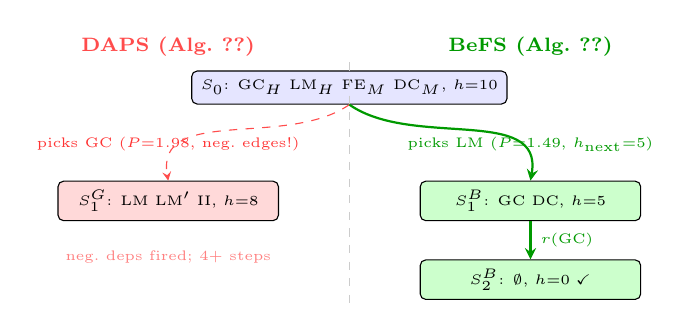
\begin{tikzpicture}[
  st/.style={draw, rectangle, rounded corners=2pt,
    minimum width=2.8cm, minimum height=0.42cm,
    text centered, font=\tiny},
  root/.style={st, fill=blue!10},
  good/.style={st, fill=green!20},
  bad/.style={st, fill=red!15},
  arr/.style={->, >=stealth, font=\tiny}]
  \node[root] (s0) at (0,0)
    {$S_0$: GC$_H$ LM$_H$ FE$_M$ DC$_M$,\ $h{=}10$};
  % DAPS branch
  \node[font=\tiny, red!80]   at (-2.3,-0.72) {picks GC\ ($P{=}1.98$, neg.\ edges!)};
  \node[bad]  (s1g) at (-2.3,-1.44)
    {$S_1^G$: LM LM$'$ II,\ $h{=}8$};
  \node[font=\tiny, red!50]   at (-2.3,-2.15) {neg.\ deps fired; 4+ steps};
  % BFS branch
  \node[font=\tiny, green!60!black] at (2.3,-0.72) {picks LM\ ($P{=}1.49$, $h_{\text{next}}{=}5$)};
  \node[good] (s1b) at (2.3,-1.44)
    {$S_1^B$: GC DC,\ $h{=}5$};
  \node[good] (s2b) at (2.3,-2.44)
    {$S_2^B$: $\emptyset$,\ $h{=}0$\;$\checkmark$};
  % Arrows
  \draw[arr, dashed, red!70]
    (s0.south) to[out=215,in=100] (s1g.north);
  \draw[arr, thick, green!60!black]
    (s0.south) to[out=325,in=80]  (s1b.north);
  \draw[arr, thick, green!60!black]
    (s1b) -- node[right]{\tiny $r(\mathrm{GC})$} (s2b);
  % Column labels
  \node[font=\scriptsize\bfseries, red!70]        at (-2.3,0.52) {DAPS (Alg.~\ref{alg:daps})};
  \node[font=\scriptsize\bfseries, green!60!black] at ( 2.3,0.52) {BeFS (Alg.~\ref{alg:befs})};
  % Divider
  \draw[gray!40, dashed] (0,0.32) -- (0,-2.75);
\end{tikzpicture}
\caption{DAPS vs.\ BeFS ordering trace.}
\label{fig:befs}
\end{figure}

\subsection{LLM-based refactoring agent}

The harness starts each smell with a lower-cost model. After a failed attempt,
it returns the current diff, test status, current-smell status, and remaining
detections to the coding agent. After two failures, it selects a
higher-capability model. Each smell receives at most five attempts and 30 model
turns per attempt. An HTTP 429 response delays and repeats the same attempt
without consuming the attempt budget. After the fifth failure, the harness
skips the smell. It marks the case as exhausted after skipping every remaining
detection.

Every Java change triggers verification, whether it came from an edit tool,
write tool, or shell command. The harness runs the project tests and Organic.
For Maven-only inputs, it derives a Gradle build and verifies through Gradle.
It blocks direct edits to build files and whole-worktree rollback commands. The
harness moves to the next smell only when
\begin{equation}
\begin{split}
\mathrm{accept}(e,s)={}&\mathrm{javaEdit}(e)\land
\mathrm{latestVerified}(e)\\
&{}\land\mathrm{testsAcceptable}(e)\land s\notin D(e),
\end{split}
\label{eq:accept}
\end{equation}
where $e$ is the latest edit, $s$ is the assigned smell, and $D(e)$ is the
detector output after that edit. The gate is binary and has no numeric
threshold. It rejects an edit if the assigned smell remains, even when the
total smell count falls.

Actual edits can differ from predicted transitions. Redetection replaces the
prediction before the next ordering decision.

%----------------------------------------------------------------------
\section{Experiment}
%----------------------------------------------------------------------

\textit{Dataset.} The evaluation uses the Composite Refactorings 2020 dataset
of Sousa et al.~\cite{sousa2020refactoring}. It links refactorings, commits,
changed or produced program elements, and smell states from 48 Java projects.
We use its range-based construction. Refactorings by the same developer form a
composite when their affected element sets overlap across consecutive developer
commits; this overlap can extend the composite transitively. Here, range means
a commit span connected through overlapping program elements, not a source-line
range. From these composites, we select a bounded class or method scope and
check out its pre-refactoring commit. The ten buildable episodes are
range-seeded, selected-scope cases, not a random sample or an exact replay of
every full composite.

\textit{Detector-order baseline.} The harness processes smells in Organic's
native detector order without dependency-based reordering.

\textit{Planned runs.} The same harness instead uses Dependency-Aware Priority
Selection (DAPS), topological ordering, or BeFS.
Each condition uses the same detector, prompt structure, weak model, escalation
rule, attempt limit, and verification gate. We count original and introduced
smells, model turns, edit tasks, verification outcomes, token use, elapsed time,
and final CK metrics. The CK static-analysis tool~\cite{aniche2015ck}
supplies CBO for coupling, LCOM for lack of cohesion, WMC for class complexity,
and LOC for size. The experiment has one run per combination of ordering and
episode, so it does not estimate variation from model sampling.

Comparing detector-order and planned runs measures the dependency rules and
search procedure together. The harness remains fixed. Verification logs
describe its recovery from failed edits, but the experiment has no second
harness for a causal comparison.

A completed run has no remaining original or introduced smell and has final CK
output. It ends after the harness removes every detected smell. The definition
has no tunable reduction threshold. It measures smell removal under the
repository tests, not semantic equivalence.

\subsection{Completion and recovery}

The $4\times10$ matrix produced 16 successful, eight failed, and 16 aborted
runs. Case-level runs added four completed observations, giving 20 completed
runs across six episodes from four projects. BeFS contributes two observations;
each other ordering contributes six. The analysis includes failed and aborted
outcomes as well as completed runs.

\begin{table}[tb]
\centering
\footnotesize
\setlength{\tabcolsep}{3.0pt}
\begin{tabular}{@{}lrrrr@{}}
\toprule
Order & Runs & Original & Introduced & Failed verify \\
\midrule
BeFS   & 2 & 32/32  & 30/30 & 12/60 \\
DAPS   & 6 & 106/106 & 67/67 & 46/202 \\
Detector & 6 & 106/106 & 65/65 & 67/224 \\
Topo   & 6 & 106/106 & 58/58 & 46/218 \\
\midrule
Total  & 20 & 350/350 & 220/220 & 171/704 \\
\bottomrule
\end{tabular}
\caption{Smell removal and failed intermediate verifications in completed
runs. Fractions show fixed/observed smells and failed/total
verifications.}
\label{tab:completion}
\end{table}

Every completed run removed all detected smells, including those introduced
during editing. Completion often required more than one edit. Compilation
failed during 171 of 704 verification attempts (24.3\%).
Fourteen of 20 runs had at least one failure. Eight runs needed a second or
third attempt for at least one smell, and three reached the third attempt. No
completed run recorded a test-case failure; final verification passed in all
20. These tests may still miss behavioural faults.

Three runs switched to the stronger model, all on the same PhiCode episode.
The stronger model used 34 of 3,594 model turns and 93,388 of 20,811,212
tokens. Since all switches occurred in one episode, these data do not isolate
the effect of escalation.

\begin{figure*}[tb]
\centering
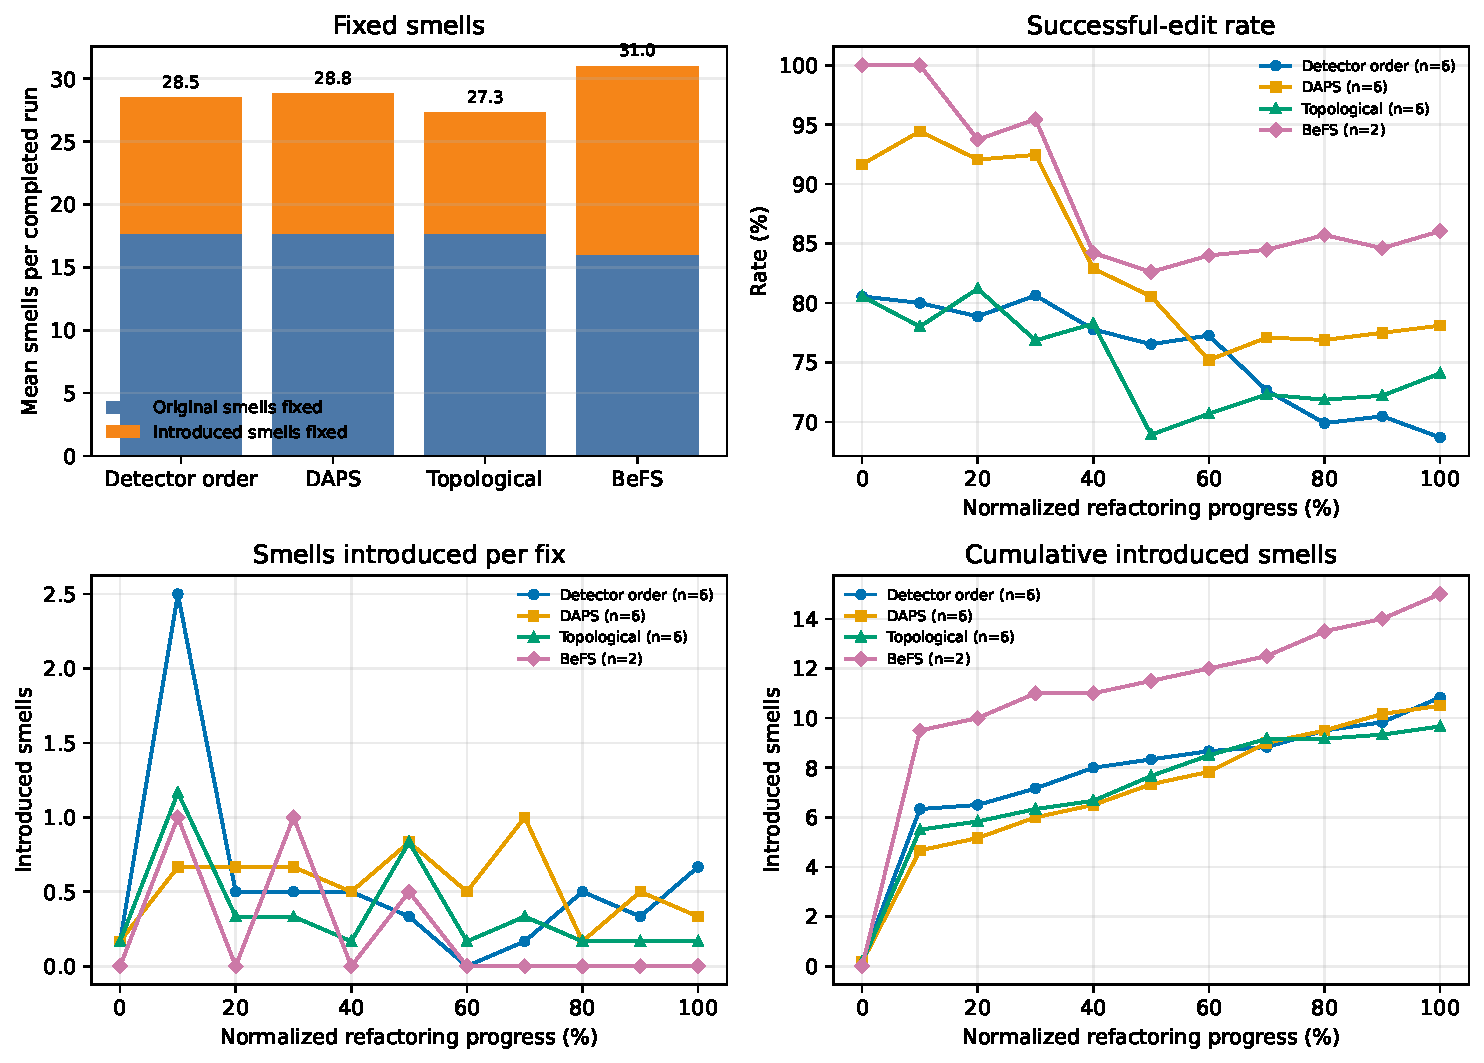
\includegraphics[width=\textwidth]{figures/aggregate_smell_metrics.pdf}
\caption{Smell statistics averaged across completed cases for each planner.
The fixed-smell panel reports mean counts per run. The trajectory panels
normalise each run from 0\% to 100\% progress and average values at
ten-percentage-point intervals. Detector-order runs, DAPS, and topological
ordering each have six cases; BeFS has two.}
\label{fig:aggregate-smell-metrics}
\end{figure*}

Fig.~\ref{fig:aggregate-smell-metrics} separates original smells from smells
introduced during refactoring. Topological ordering fixed 9.7 introduced smells
per completed run on average, compared with 10.8 for detector order and 11.2
for DAPS. BeFS averaged 15.0 across its two completed cases. Every introduced
smell in these runs was later removed.

\subsection{Ordering outcomes and overhead}

\begin{figure*}[tb]
\centering
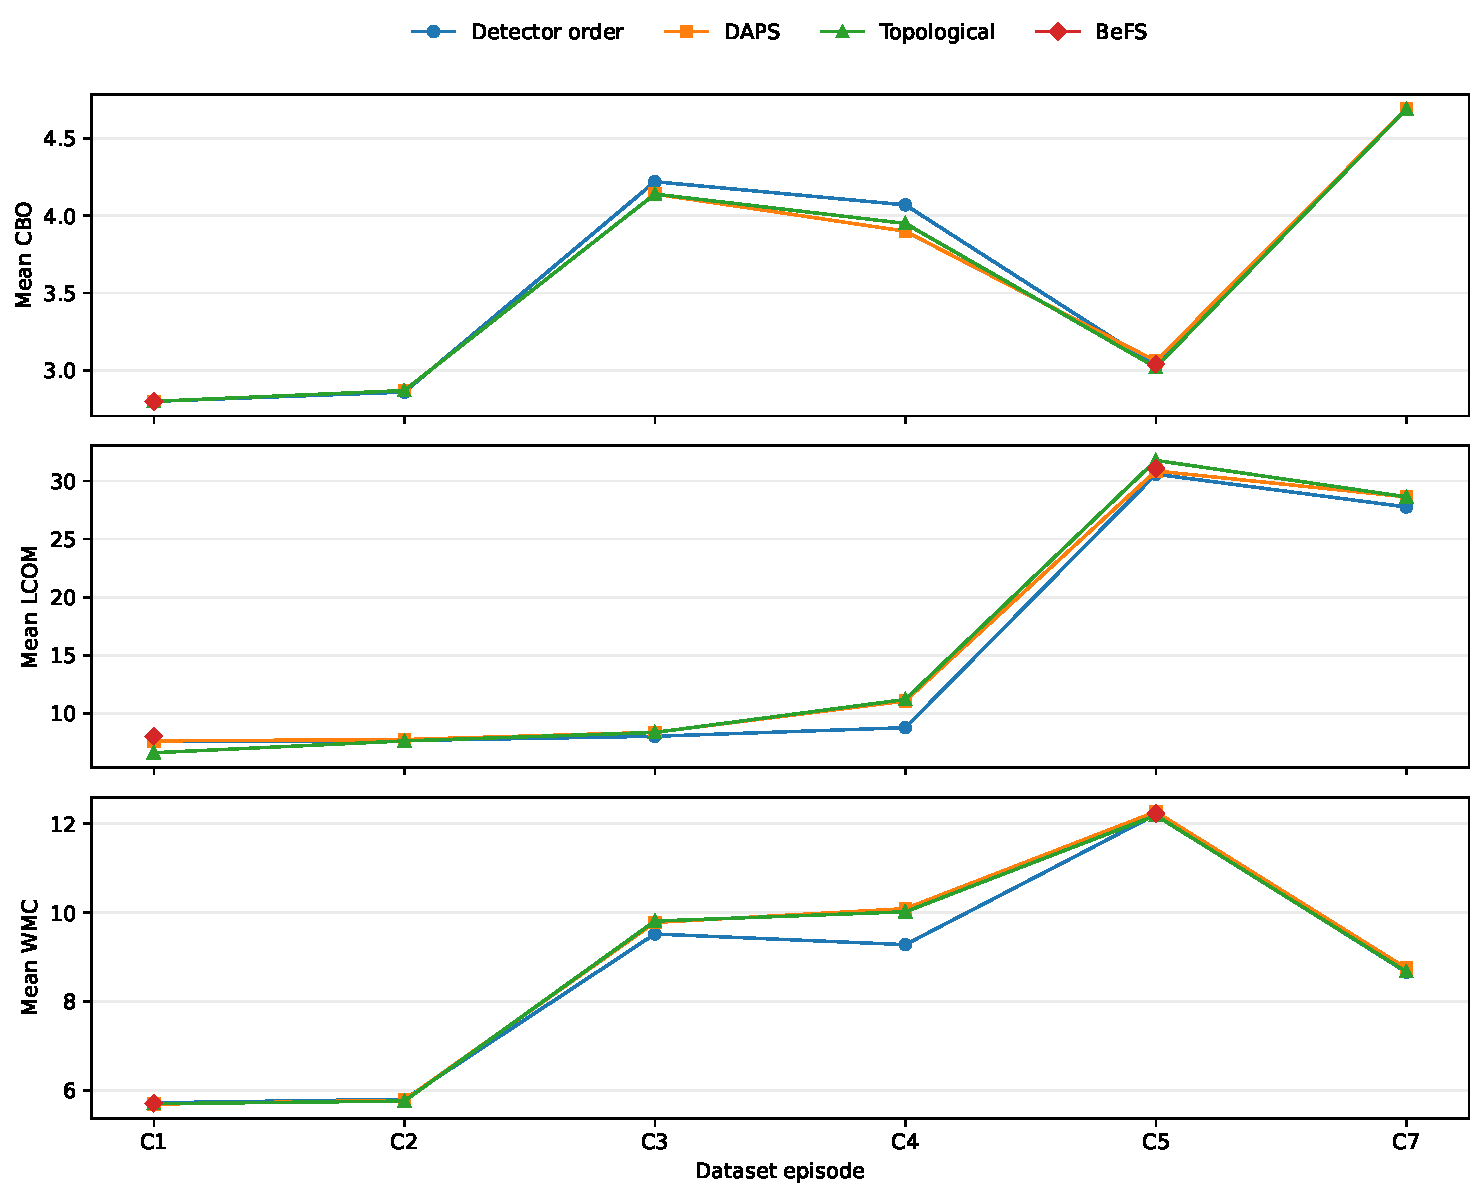
\includegraphics[width=\textwidth]{figures/final_design_metrics.pdf}
\caption{Final design metrics from the experiment report. Each marker is one
completed combination of planner and episode. Missing markers denote
unavailable runs.}
\label{fig:final-design-metrics}
\end{figure*}

\begin{figure*}[tb]
\centering
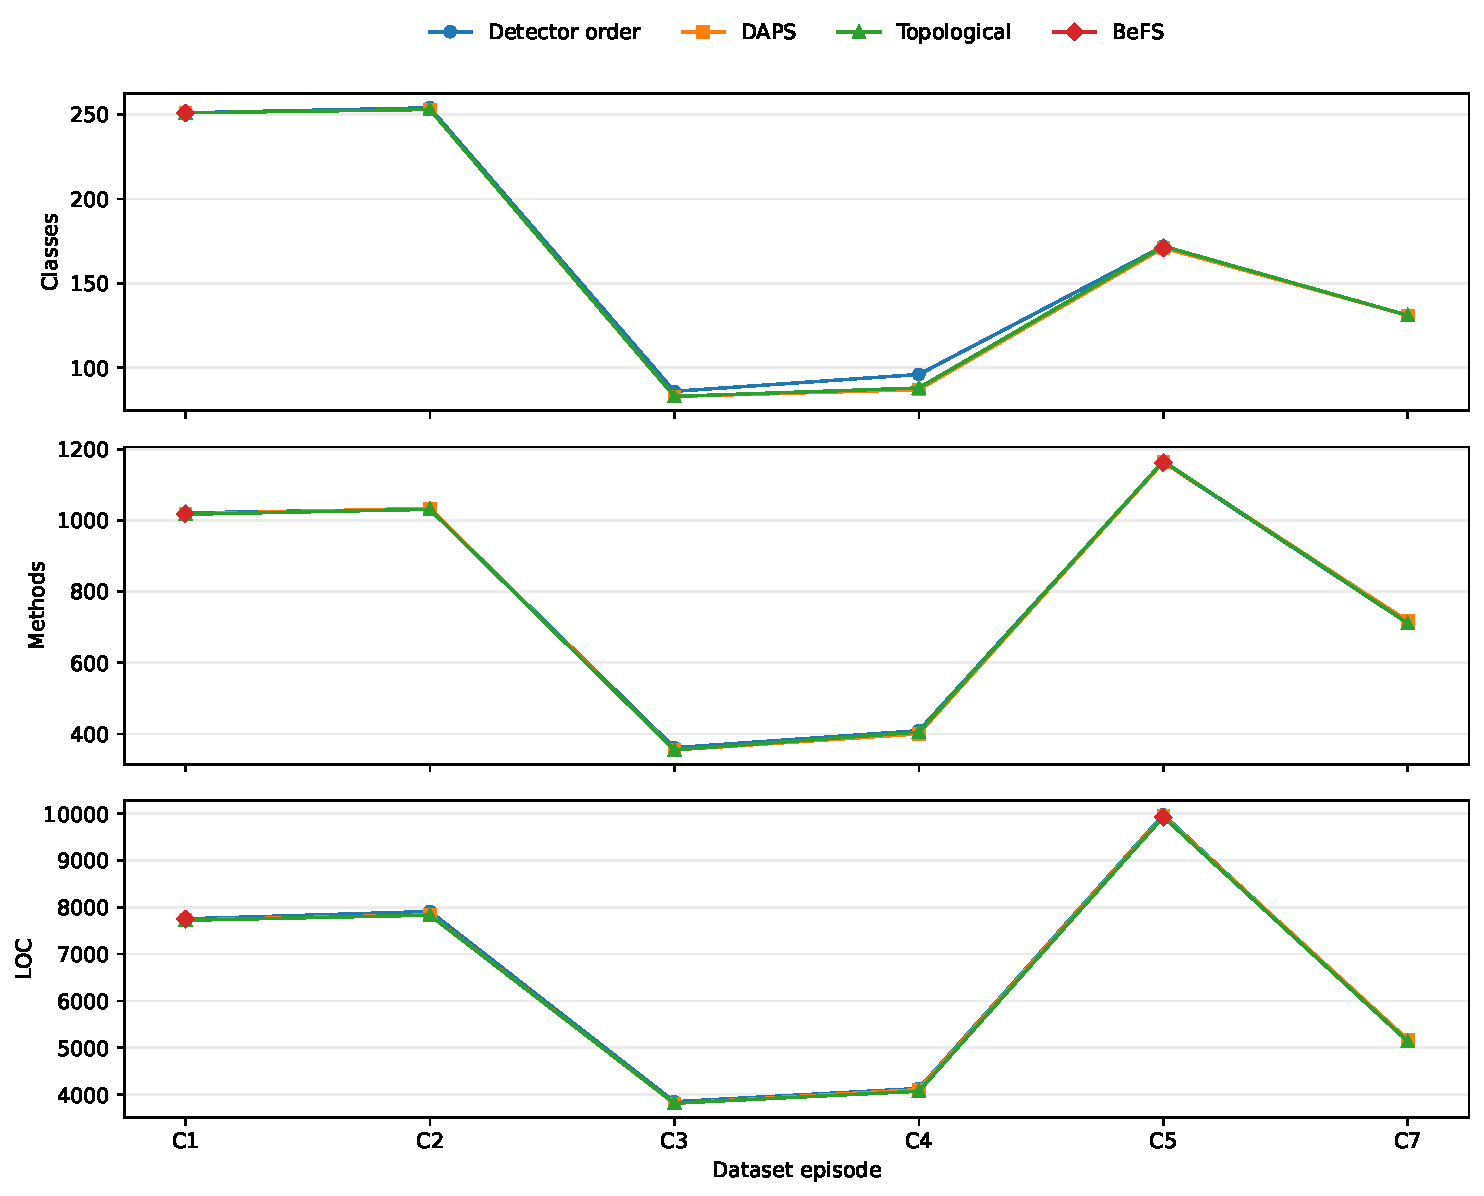
\includegraphics[width=\textwidth]{figures/final_size_metrics.pdf}
\caption{Final class count, method count, and LOC from the experiment report.
The values remain close across orderings within each completed episode.}
\label{fig:final-size-metrics}
\end{figure*}

\begin{table}[tb]
\centering
\footnotesize
\setlength{\tabcolsep}{4.0pt}
\begin{tabular}{@{}lrrrrr@{}}
\toprule
Order & Runs & Tasks & Turns & Tokens & Minutes \\
\midrule
BeFS   & 2 & 39  & 366   & 1,571,971 & 67.7 \\
DAPS   & 6 & 95  & 1,035 & 6,263,115 & 174.3 \\
Detector & 6 & 92  & 1,090 & 6,661,949 & 144.8 \\
Topo   & 6 & 102 & 1,103 & 6,314,177 & 146.7 \\
\midrule
Total  & 20 & 328 & 3,594 & 20,811,212 & 533.5 \\
\bottomrule
\end{tabular}
\caption{Observed work and token use for completed runs. BeFS totals
cover two episodes and are not directly comparable with the six-episode
totals.}
\label{tab:overhead}
\end{table}

The detector-order, DAPS, and topological conditions cover the same six completed
episodes. DAPS used the fewest model turns (1,035) and the fewest tokens
(6,263,115). Detector-order runs had the lowest elapsed time (144.8 minutes).
Topological order introduced the fewest smells (58, versus 65 for detector
order and 67 for DAPS).

BeFS covers two episodes rather than six, so we compare the orderings on the two
shared episodes. BeFS introduced 30 smells and used 39 edit tasks. DAPS
introduced 23 and used 32, detector order introduced 31 and used 33, and
topological ordering introduced 25 and used 42. BeFS introduced fewer smells
than detector order and used fewer tasks than topological ordering. DAPS
introduced fewer smells and used fewer tasks than BeFS.

The detector-order condition provides the CK baseline for comparing final
states. Across the six episodes shared by detector order, DAPS, and topological
execution, most final values changed little. Relative to the detector-order
value, the cross-planner spread was at most 4.2\% for CBO, 8.7\% for WMC, 1.4\% for LOC,
9.4\% for class count, and 2.2\% for method count. LCOM was also close in four
episodes, with spreads from 1.6\% to 4.2\%, but differed by 19.0\% and 27.7\%
in two episodes. Ordering had a clearer effect on intermediate outcomes than on
the final CK values.

%----------------------------------------------------------------------
\section{Discussion and Future Work}
%----------------------------------------------------------------------

\textbf{(RQ1) Planner choice.} In the initial $4\times10$ matrix, detector
order, DAPS, and topological execution each completed five cases; BeFS completed
one. Across the six episodes later completed by detector order, DAPS, and
topological execution, they used 92, 95, and 102 edit tasks respectively. DAPS
used 1,035 model turns, compared with 1,090 for detector order and 1,103 for
topological ordering. The planners differed in work and token use, but no
planner led every outcome. The single run per cell and unequal completed
coverage prevent a causal ranking.

\textbf{(RQ2) Dependency rules.} The experiment does not isolate the rules.
The detector-order condition omits dependency-based planning. DAPS, topological
ordering, and BeFS combine the rules with different search procedures. A clean
test would run each algorithm twice, once with dependency edges and once
without them.

\textbf{(RQ3) Predicted and observed dependencies.} The same rule graph led to
different smell sequences. Across the six matched episodes,
topological ordering introduced 58 smells, detector order 65, and DAPS
67. On the two episodes shared with BeFS, DAPS introduced 23, topological
ordering 25, BeFS 30, and detector order 31. Dependency rules alone did
not guarantee fewer introduced smells. The planner determined which edges
became relevant, and redetection showed which predicted effects occurred.
Because the rules and search procedure change together, these data cannot
assign each introduced smell to one factor.

\textbf{(RQ4) Structural quality.} Final CBO, WMC, LOC, class count, and method
count remained close across algorithms. LCOM differed more in two episodes,
but no planner was consistently lower. The logs contain Organic measurements
after each edit, but CK measurements only at run completion. They support a
comparison of final code states, not a step-by-step CK trajectory. Measuring
that trajectory requires CK collection after every accepted refactoring.

\textbf{Harness recovery.} Fourteen completed runs encountered at least one
compilation failure, yet all 20 completed runs removed every detected smell.
The harness reported the failure, retried the same smell, and switched to a
stronger model after two failures. These logs show recovery within this
harness, not an advantage over another execution system.

\subsection{Limitations and Responsible AI}

The ten episodes are a selected Java-only subset of the Sousa-derived dataset.
The evaluation excludes other projects and programming languages. Four
episodes yielded no completed observation, and coverage differs across
orderings. The dependency catalogue is incomplete, and measured edits do not
calibrate its edge probabilities. Organic findings and CK metrics help identify
structurally problematic code.

The task is behaviour-preserving refactoring. The harness changes production
code and keeps the repository tests fixed. Passing those tests does not prove
semantic equivalence or adequate coverage. Future work should use
change-focused coverage and mutation testing to check whether the tests execute
modified code and detect injected faults. A developer must review the diff,
detector output, and test result before merging a patch. The system does not
deploy generated changes.

External model providers may receive source code. Users must apply their
repository privacy and data-processing rules. Reproduction requires the pinned
repository commits, detector and extension versions, model configuration, and
execution limits. Source code, experiment configuration, and figure-generation
data are available at
\url{https://github.com/hpietukhin/refactoring-with-llms}.

Each ordering algorithm should be run with and without dependency edges. This
would separate the rules from the search procedure. Frequencies measured from
actual edits could then calibrate the catalogue edges.

\section{Conclusion}

We integrated dependency-aware smell ordering with a coding-agent harness. The
extension verifies each Java edit, returns the result to the model, retries
failed smells, and escalates the model after two failures. Across 20 completed
runs, it removed all 350 initial and 220 introduced detections despite 171 failed
intermediate compilations. The harness recovered across edits but did not
succeed on every edit or case. DAPS used the fewest model turns and the
fewest tokens. Detector-order runs had the shortest elapsed time, while
topological ordering introduced the fewest smells across their six completed
episodes. On the two episodes shared with BeFS, it introduced fewer smells than
detector order and used fewer edit tasks than topological ordering. Final
CK metrics were mostly similar across planners. The experiment changes the
rules and algorithm together, so it cannot assign their effects separately.

\section*{Acknowledgement}
This work was supported by the European Union NextGenerationEU via the Recovery
and Resilience Plan for Slovakia through the project\
"InnovAIte Slovakia, Illuminating Pathways for AI-Driven Breakthroughs"
(No.~09I02-03-V01-00029).

\bibliographystyle{IEEEtran}
\bibliography{references}

\end{document}
